% =====================================================================
%  Báo cáo Project 2 — Nhận diện & mapping 2D trận đấu bóng đá từ video
%  Biên dịch: khuyến nghị XeLaTeX hoặc LuaLaTeX (font Unicode tiếng Việt).
%    - pdfLaTeX: cần gói vntex; giữ nguyên phần babel bên dưới.
%    - XeLaTeX : bỏ 3 dòng inputenc/fontenc/babel, dùng khối fontspec (đã chú thích).
% =====================================================================
\documentclass[12pt,a4paper]{article}

% --- Tiếng Việt (pdfLaTeX + vntex) ---
\usepackage[utf8]{inputenc}
\usepackage[T5]{fontenc}
\usepackage[vietnamese]{babel}
% --- Nếu dùng XeLaTeX/LuaLaTeX, thay 3 dòng trên bằng: ---
% \usepackage{fontspec}
% \usepackage{polyglossia}\setmainlanguage{vietnamese}
% \setmainfont{Times New Roman}

\usepackage[a4paper,margin=2.5cm]{geometry}
\usepackage{amsmath,amssymb}
\usepackage{graphicx}
\usepackage{booktabs}
\usepackage{caption}
\usepackage{enumitem}
\usepackage{xcolor}
\usepackage{float}
\usepackage[hidelinks]{hyperref}
\usepackage{tikz}
\usetikzlibrary{positioning,arrows.meta}
\graphicspath{{figures/}{metrics/}}

% --- Màu cho sơ đồ pipeline ---
\definecolor{cgreen}{HTML}{2E7D46}
\definecolor{cpurple}{HTML}{6D4AA7}
\definecolor{cred}{HTML}{C0392B}
\definecolor{cteal}{HTML}{12869B}
\definecolor{corange}{HTML}{C96A1B}
\definecolor{cblue}{HTML}{3A6EA5}
\definecolor{csteel}{HTML}{4B5566}
\tikzset{
  box/.style={rectangle, rounded corners=2pt, draw=black!35, thick, fill=#1,
    text=white, align=center, font=\small, minimum height=1.05cm,
    text width=2.35cm, inner sep=3pt},
  io/.style={rectangle, rounded corners=3pt, draw=black!45, dashed, thick,
    fill=white, text=black, align=center, font=\small, minimum height=1.05cm,
    text width=1.9cm, inner sep=3pt},
  flow/.style={-{Latex[length=2mm,width=1.6mm]}, thick, draw=black!55},
}

\setlength{\parskip}{0.4em}
\renewcommand{\arraystretch}{1.2}

\begin{document}

% ============================ TRANG BÌA ============================
\begin{titlepage}
\centering
{\large ĐẠI HỌC BÁCH KHOA HÀ NỘI\par}
{\large TRƯỜNG CÔNG NGHỆ THÔNG TIN \& TRUYỀN THÔNG\par}
\vspace{3cm}
{\Huge\bfseries Báo Cáo Project\par}
\vspace{1cm}
{\Large Đề tài: Nhận diện và mapping 2D\\[4pt] trận đấu bóng đá từ video\par}
\vspace{2cm}
\begin{flushleft}
\hspace{3cm}\begin{tabular}{ll}
Học phần: & Project 2\\[4pt]
Giảng viên hướng dẫn: & Nguyễn Quốc Tuấn\\[4pt]
Sinh viên thực hiện: & Đỗ Ngọc Hoàng Hải\\[4pt]
Mã số sinh viên: & 20230026\\
\end{tabular}
\end{flushleft}
\vfill
{\large Hà Nội, năm 2026\par}
\end{titlepage}

\tableofcontents
\newpage

% ============================ 1. MỤC TIÊU ============================
\section{Mục tiêu đề tài}
Đề tài xây dựng một hệ thống thị giác máy tính (Computer Vision) phân tích cảnh quay
bóng đá phát sóng từ \emph{một} camera (broadcast), gồm hai mức:
\begin{itemize}[leftmargin=1.4em]
  \item \textbf{Nhận diện} bốn đối tượng trên sân: cầu thủ (\textit{player}), bóng
        (\textit{ball}), thủ môn (\textit{goalkeeper}) và trọng tài (\textit{referee}).
  \item \textbf{Phân tích chiến thuật}: phân biệt hai đội theo màu áo; dựng
        \textbf{bản đồ 2D (radar)} chiếu vị trí cầu thủ và bóng nhìn từ trên xuống;
        vẽ \textbf{biểu đồ Voronoi} thể hiện vùng kiểm soát không gian của hai đội;
        và \textbf{ước lượng tốc độ} di chuyển tức thời (km/h) của từng cầu thủ.
\end{itemize}
Đầu vào có thể là ảnh hoặc video; đầu ra là khung hình được chú giải kèm radar 2D và
biểu đồ Voronoi hiển thị đồng thời theo phong cách đồ hoạ thể thao. Toàn bộ mã nguồn
được đóng gói thành package Python \texttt{football\_analysis} chạy được offline
(weights \texttt{.pt} local) hoặc qua Roboflow API.

% ============================ 2. DỮ LIỆU ============================
\section{Dữ liệu}
Dự án sử dụng hai bộ dữ liệu riêng cho hai bài toán, quản lý qua nền tảng Roboflow:
\begin{itemize}[leftmargin=1.4em]
  \item \textbf{Phát hiện đối tượng}: bộ \textit{soccernet} với bốn lớp, chia tập huấn
        luyện khoảng 1.988 ảnh / 29.982 đối tượng và tập kiểm định khoảng 1.989 ảnh /
        28.213 đối tượng.
  \item \textbf{Keypoint sân}: bộ \textit{football-field-detection} gồm 32 điểm mốc đặc
        trưng trên sân (giao điểm/góc của các vạch kẻ), dùng để ước lượng phép biến đổi
        phối cảnh (homography).
\end{itemize}

% ============================ 3. HUẤN LUYỆN ============================
\section{Huấn luyện hai mô hình nhận diện}
\textbf{Mô hình phát hiện cầu thủ/bóng.} Dựa trên kiến trúc \textbf{YOLOv11s}, huấn luyện
theo lối transfer learning từ trọng số \texttt{yolo11s.pt} trong 32 epoch, kích thước
ảnh đầu vào 1280\,px, batch 32; quá trình huấn luyện được theo dõi bằng Weights \& Biases.

\textbf{Mô hình keypoint sân.} Sử dụng \textbf{YOLOv11s-pose} (bài toán pose/keypoint),
huấn luyện 100 epoch, ảnh 640\,px, batch 32, tắt augmentation mosaic. Mô hình phát hiện
32 điểm mốc cố định trên sân làm cơ sở tính homography.

Cả hai mô hình được lưu thành trọng số \texttt{.pt} chạy trực tiếp trên máy (Ultralytics);
ngoài ra có thể triển khai lên Roboflow để gọi inference qua API. Pipeline hỗ trợ chọn
\emph{nguồn từng mô hình một cách độc lập} (xem mục~\ref{sec:homography}).

\begin{figure}[H]\centering
  
\includegraphics[width=.8\textwidth]{figures/Players Detection/train_batch0.jpg}
  \caption{Một batch dữ liệu huấn luyện mô hình phát hiện (kèm augmentation), với
           nhãn bốn lớp \textit{player}, \textit{ball}, \textit{goalkeeper}, \textit{referee}.}
\end{figure}

% ============================ 4. PIPELINE ============================
\section{Pipeline suy luận (inference)}
Phần này mô tả chi tiết luồng xử lý đưa từ một khung hình thô thành khung hình chú giải
đầy đủ kèm radar và Voronoi. Sơ đồ tổng quan ở Hình~\ref{fig:pipeline}.

\begin{figure}[H]\centering
  \includegraphics[width=\textwidth]{figures/pipeline_diagram.png}
\caption{Kiến trúc pipeline hai lượt. Song song ở Lượt~1 còn có \emph{Ball Tracker}
(toạ độ ảnh), \emph{keypoint sân} (YOLOv11s-pose) và \emph{optical flow} (chuyển động
camera $dH$) cùng ghi vào records; xem mục~\ref{sec:homography}.}
\label{fig:pipeline}
\end{figure}

\subsection{Kiến trúc hai lượt (two-pass)}
Một số hiệu chỉnh không thể thực hiện chính xác nếu chỉ xử lý tuần tự từng khung hình,
vì chúng cần thông tin \emph{toàn cục} của cả đoạn (ví dụ: biết bóng rơi ở đâu mới vẽ
được quỹ đạo thẳng; làm mượt \emph{có tâm} cần cả khung hình tương lai). Do đó pipeline
video được tổ chức thành hai lượt, và mô hình chỉ chạy suy luận \emph{một lần}:
\begin{itemize}[leftmargin=1.4em]
  \item \textbf{Lượt 1 -- phân tích}: chạy hai mô hình trên từng khung hình và lưu lại
        dữ liệu gọn nhẹ cho mỗi khung (hộp giới hạn, ID, lớp/đội, quan sát keypoint sân,
        và chuyển động camera liên khung ước lượng bằng optical flow). Không lưu ảnh nên
        nhẹ bộ nhớ. \emph{Toạ độ sân được tính ở lượt 2.}
  \item \textbf{Lượt 2 -- hậu kỳ và vẽ}: làm mượt chuỗi keypoint theo thời gian rồi fit
        lại homography từng khung, xử lý hậu kỳ trên toàn bộ chuỗi (chống nhấp nháy
        minimap, làm thẳng quỹ đạo bóng, làm mượt tốc độ) rồi vẽ lại khung hình mà không
        suy luận lại.
\end{itemize}

\subsection{Phát hiện và theo dõi đối tượng}
Mỗi khung hình được đưa qua mô hình phát hiện để thu các đối tượng của bốn lớp. Quả bóng
được tách riêng; nhóm người (cầu thủ, thủ môn, trọng tài) được lọc trùng bằng
\textbf{Non-Maximum Suppression} (IoU 0.5, không phân biệt lớp) rồi đưa qua thuật toán
theo dõi \textbf{ByteTrack} để gán một định danh (ID) ổn định cho từng người xuyên suốt
các khung hình. ID ổn định là nền tảng cho mọi bước về sau (chống nhấp nháy đội, tính
tốc độ, chống flicker minimap). Mô hình detection được suy luận ở \emph{đúng độ phân giải
huấn luyện} (1280\,px) thay vì mặc định 640\,px của thư viện --- nếu để 640\,px sẽ sót
nhiều cầu thủ ở xa (đo trên video mẫu: 640\,px thấy 13--19 người/khung, 1280\,px thấy
22--25).

\subsection{Phân đội và gán thủ môn}
Việc phân biệt hai đội dựa trên màu áo, gồm các bước:
\begin{itemize}[leftmargin=1.4em]
  \item \textbf{Trích đặc trưng}: với mỗi cầu thủ, cắt vùng \emph{thân áo} (nửa trên hộp
        giới hạn, tỉ lệ $0\!-\!0{,}55$ chiều cao) để loại nhiễu từ quần, chân và mặt cỏ;
        vùng này được mã hoá thành vector đặc trưng bằng mô hình embedding ảnh
        \textbf{SigLIP}.
  \item \textbf{Phân cụm}: giảm chiều các vector bằng \textbf{UMAP} rồi phân cụm
        \textbf{KMeans} thành hai nhóm tương ứng hai đội. Bộ phân loại được \emph{fit
        trước} trên các crop thu thập từ chính nguồn đầu vào (lấy mẫu theo bước
        \texttt{fit\_stride}).
  \item \textbf{Chống nhấp nháy nhãn đội}: dự đoán theo từng khung hình rất dễ dao động,
        nên hệ thống lưu lịch sử nhãn theo ID và xuất ra nhãn theo \textbf{bỏ phiếu đa số}
        trên một cửa sổ thời gian, kèm cơ chế \textbf{hysteresis} (chỉ đổi đội khi phe mới
        thực sự áp đảo, ngưỡng \texttt{switch\_ratio}).
  \item \textbf{Gán thủ môn}: thủ môn (áo khác hai đội) được gán về đội có \emph{trọng tâm
        cầu thủ gần hơn} trong toạ độ ảnh, và cũng được làm mượt theo ID như trên.
\end{itemize}

\subsection{Ánh xạ phối cảnh (homography) và bản đồ 2D}
\label{sec:homography}
Từ 32 keypoint sân do mô hình pose phát hiện, hệ thống ước lượng phép biến đổi phối cảnh
$H$ đưa toạ độ điểm trên ảnh về toạ độ sân chuẩn nhìn từ trên xuống. Vì mặt sân phẳng,
một điểm sân $(x,y)$ và ảnh của nó $(u,v)$ liên hệ qua ma trận $3\times3$:
\begin{equation}
  \begin{bmatrix} u' \\ v' \\ w' \end{bmatrix}
  = H \begin{bmatrix} x \\ y \\ 1 \end{bmatrix},\qquad
  u=\frac{u'}{w'},\; v=\frac{v'}{w'} .
\end{equation}
Nguyên tắc thiết kế xuyên suốt là \textbf{``làm mượt phép đo, không làm mượt mô hình''}
--- làm mượt vị trí keypoint (luôn nằm trong ảnh) thay vì làm mượt trực tiếp ma trận $H$
hay tham số camera. Khối này gồm bốn bước:

\paragraph{(1) Fit bền vững từng khung.} $H$ được fit \emph{least-squares trên toàn bộ}
keypoint quan sát rồi mới loại các điểm có sai số tái chiếu (reprojection error) lệch quá
xa so với fit toàn cục --- ngưỡng thích nghi $\max(2\cdot\texttt{ransac\_px},\,3\cdot
\mathrm{median}(\text{res}))$ --- và fit lại. Cách này giữ được ``baseline'' trải rộng
khắp sân, thay cho RANSAC: khi nhiễu keypoint ($\sim$15--35\,px) vượt ngưỡng, RANSAC dễ
khoá vào một cụm 5--6 điểm sát nhau tự nhất quán rồi loại hết các điểm trải rộng, khiến
$H$ ngoại suy lệch nhiều mét mà cổng kiểm tra reprojection không phát hiện được.

\paragraph{(2) Làm mượt có tâm theo thời gian.} Chuỗi vị trí ảnh của \emph{từng} keypoint
qua các khung được lọc trung vị (chặn outlier đơn lẻ) và làm mượt \emph{có tâm} bằng
\textbf{Savitzky-Golay bậc 2} --- bám được chuyển động lia nhanh mà không trễ như trung
bình trượt nhân quả (khả thi nhờ kiến trúc hai lượt). Keypoint chỉ được lấp \emph{khoảng
trống ngắn} trong phạm vi thực sự được quan sát, \emph{không bao giờ ngoại suy} ra ngoài
khung hình.

\paragraph{(3) Fit lại homography.} Sau khi làm sạch, $H$ được fit lại từng khung từ
keypoint đã làm mượt (least-squares, không cần cắt outlier nữa vì dữ liệu đã sạch), kèm
cổng chặn reprojection error tối đa.

\paragraph{(4) Bắc cầu quãng mất sân bằng dead-reckoning quang học.} Khung hình model mất
sân (mờ do lia nhanh) được bù bằng chuyển động camera liên khung: vì camera phát sóng
quay/zoom quanh trục cố định, chuyển động giữa hai khung là một homography toàn cục $dH$
ước lượng từ optical flow toàn khung hình (Shi--Tomasi + Lucas--Kanade + RANSAC) mà không
cần thấy vạch sân. Cập nhật $H_t = dH\cdot H_{t-1}$ giúp bản đồ tiếp tục bám camera qua
quãng mù, thay cho việc đóng băng $H$ cũ (gây lệch nhiều mét) hay nội suy ma trận (gây
méo dần); thiếu cả optical flow mới giữ $H$ hợp lệ gần nhất.

Chân mỗi cầu thủ (điểm giữa cạnh đáy hộp) và vị trí bóng được chiếu qua $H^{-1}$ lên sân
chuẩn để dựng minimap. Vì $H$ fit trực tiếp từ quan sát, nó tự hấp thụ sai lệch hệ thống
của thiết bị thật (méo ống kính, template sân chuẩn khác kích thước sân thật). Hệ thống
còn hỗ trợ \textbf{chế độ hybrid} chọn nguồn từng mô hình riêng biệt: phát hiện cầu thủ
bằng weights tự huấn luyện chạy local, còn keypoint sân gọi mô hình hosted huấn luyện
trên dataset lớn --- trên video mẫu, mô hình sân hosted bám sân 750/750 khung hình (so
với 588/750 của mô hình tự huấn luyện), cho bản đồ 2D ổn định hơn rõ rệt.

\subsection{Biểu đồ Voronoi}
Song song với radar, hệ thống vẽ biểu đồ Voronoi trên mặt sân chuẩn: mỗi điểm trên sân
được tô màu theo đội có cầu thủ gần nhất, thể hiện trực quan vùng kiểm soát không gian của
hai đội. Bản đồ dùng kỹ thuật \emph{chuyển màu mượt} (hàm $\tanh$) giữa hai vùng thay vì
ranh giới cứng để dễ quan sát. Để chống nhấp nháy trên minimap, chuỗi vị trí sân của từng
track được hậu xử lý ở lượt hai: lấp khoảng trống ngắn khi detection chớp tắt ($\le 1$\,s,
chỉ trong khoảng track thực sự được quan sát) và làm mượt có tâm (trung vị + Savitzky-Golay);
track mất hẳn thì chấm biến mất thay vì vẽ ``bóng ma''.

\subsection{Ước lượng tốc độ cầu thủ}
Tốc độ tức thời của mỗi cầu thủ được tính trên \emph{toạ độ sân} (đơn vị thực, không phải
pixel): lấy quãng đường di chuyển theo từng ID chia cho thời gian (suy ra từ tốc độ khung
hình) rồi quy đổi sang km/h. Do số đo rất nhạy với nhiễu, hệ thống áp dụng:
\begin{itemize}[leftmargin=1.4em]
  \item làm sạch các bước nhảy phi lý (do tráo ID giữa hai người gần nhau, ngưỡng vận tốc
        tối đa \texttt{max\_player\_ms});
  \item làm mượt vị trí theo từng track rồi tính \emph{vi sai trung tâm} trên một cửa sổ
        thời gian thay vì chênh lệch hai khung liền kề;
  \item chặn trên giá trị tối đa (\texttt{max\_kmh}) để loại các đỉnh nhiễu còn sót.
\end{itemize}

\subsection{Xử lý quả bóng: chống nhấp nháy và làm thẳng quỹ đạo}
Quả bóng là đối tượng khó nhất nên cần các cơ chế riêng:
\begin{itemize}[leftmargin=1.4em]
  \item \textbf{Chống nhấp nháy (toạ độ ảnh)}: chọn detection gần vị trí trước đó nhất
        (loại hộp nhiễu ở xa, ngưỡng \texttt{max\_jump}), giữ vị trí cũ vài khung khi mất
        dấu (coast), và làm mượt bằng EMA; mất dấu quá lâu thì quên vị trí để lần phát
        hiện sau bắt lại từ đầu.
  \item \textbf{Làm thẳng quỹ đạo bóng bay trên bản đồ 2D}: homography giả định mọi điểm
        nằm trên mặt sân, nên khi bóng bay cao, điểm chiếu xuống đất bị ``vọt'' ra xa tạo
        vòng cung sai. Giải pháp là mô hình hoá quỹ đạo bóng thành đường gấp khúc nối
        \emph{các lần chạm bóng}: tại lần chạm, bóng sát mặt sân nên phép chiếu đáng tin;
        giữa hai lần chạm (kể cả khi bay) vị trí được nội suy thẳng. Phát hiện ``chạm
        bóng'' dựa trên khoảng cách từ bóng tới bàn chân gần nhất trong ảnh. Khi bóng mất
        dấu quá lâu ($>$ \texttt{max\_gap\_s}), bóng được \emph{ẩn} khỏi bản đồ thay vì
        đóng băng ở vị trí cuối.
\end{itemize}

\subsection{Tổng hợp khung hình}
Khung hình cuối được tạo bằng cách: vẽ ellipse dưới chân người (màu theo đội), tam giác
trên quả bóng, nhãn tốc độ km/h (hoặc \texttt{\#ID} cho trọng tài); sau đó ghép radar
(đặt ở giữa, sát mép dưới) và Voronoi (đặt bên cạnh) chồng lên khung hình theo bố cục gợi
nhớ đồ hoạ trong game thể thao. Mỗi lớp overlay (radar, Voronoi, quả bóng) đều bật/tắt
độc lập; ngoài ra có tuỳ chọn điều chỉnh FPS video kết quả (giữ nguyên thời lượng).

% ============================ 5. KẾT QUẢ ============================
\section{Kết quả và đánh giá}

\subsection{Mô hình phát hiện cầu thủ/bóng (trên tập kiểm định)}
Tốc độ suy luận khoảng 4--5\,ms mỗi ảnh trên GPU. Mô hình nhận diện người (cầu thủ, trọng
tài, thủ môn) rất tốt; quả bóng là lớp khó nhất do kích thước nhỏ, dễ bị che và chuyển
động nhanh --- đây cũng là nguyên nhân chính của hiện tượng bóng nhấp nháy mà pipeline
phải xử lý thêm.

\begin{table}[H]\centering
\caption{Kết quả mô hình YOLOv11s phát hiện bốn lớp.}
\begin{tabular}{lcccc}
\toprule
Lớp & Precision & Recall & mAP@50 & mAP@50--95 \\
\midrule
Tất cả     & 0.902 & 0.882 & 0.897 & 0.655 \\
player     & 0.965 & 0.964 & 0.985 & 0.792 \\
referee    & 0.941 & 0.968 & 0.982 & 0.788 \\
goalkeeper & 0.931 & 0.934 & 0.937 & 0.696 \\
ball       & 0.772 & 0.664 & 0.686 & 0.346 \\
\bottomrule
\end{tabular}
\end{table}

\begin{figure}[H]\centering
  
\includegraphics[width=\textwidth]{figures/Players Detection/results.png}
  \caption{Quá trình huấn luyện mô hình phát hiện: các thành phần loss giảm dần và
           các chỉ số Precision/Recall/mAP tăng theo epoch.}
\end{figure}

\begin{figure}[H]\centering
  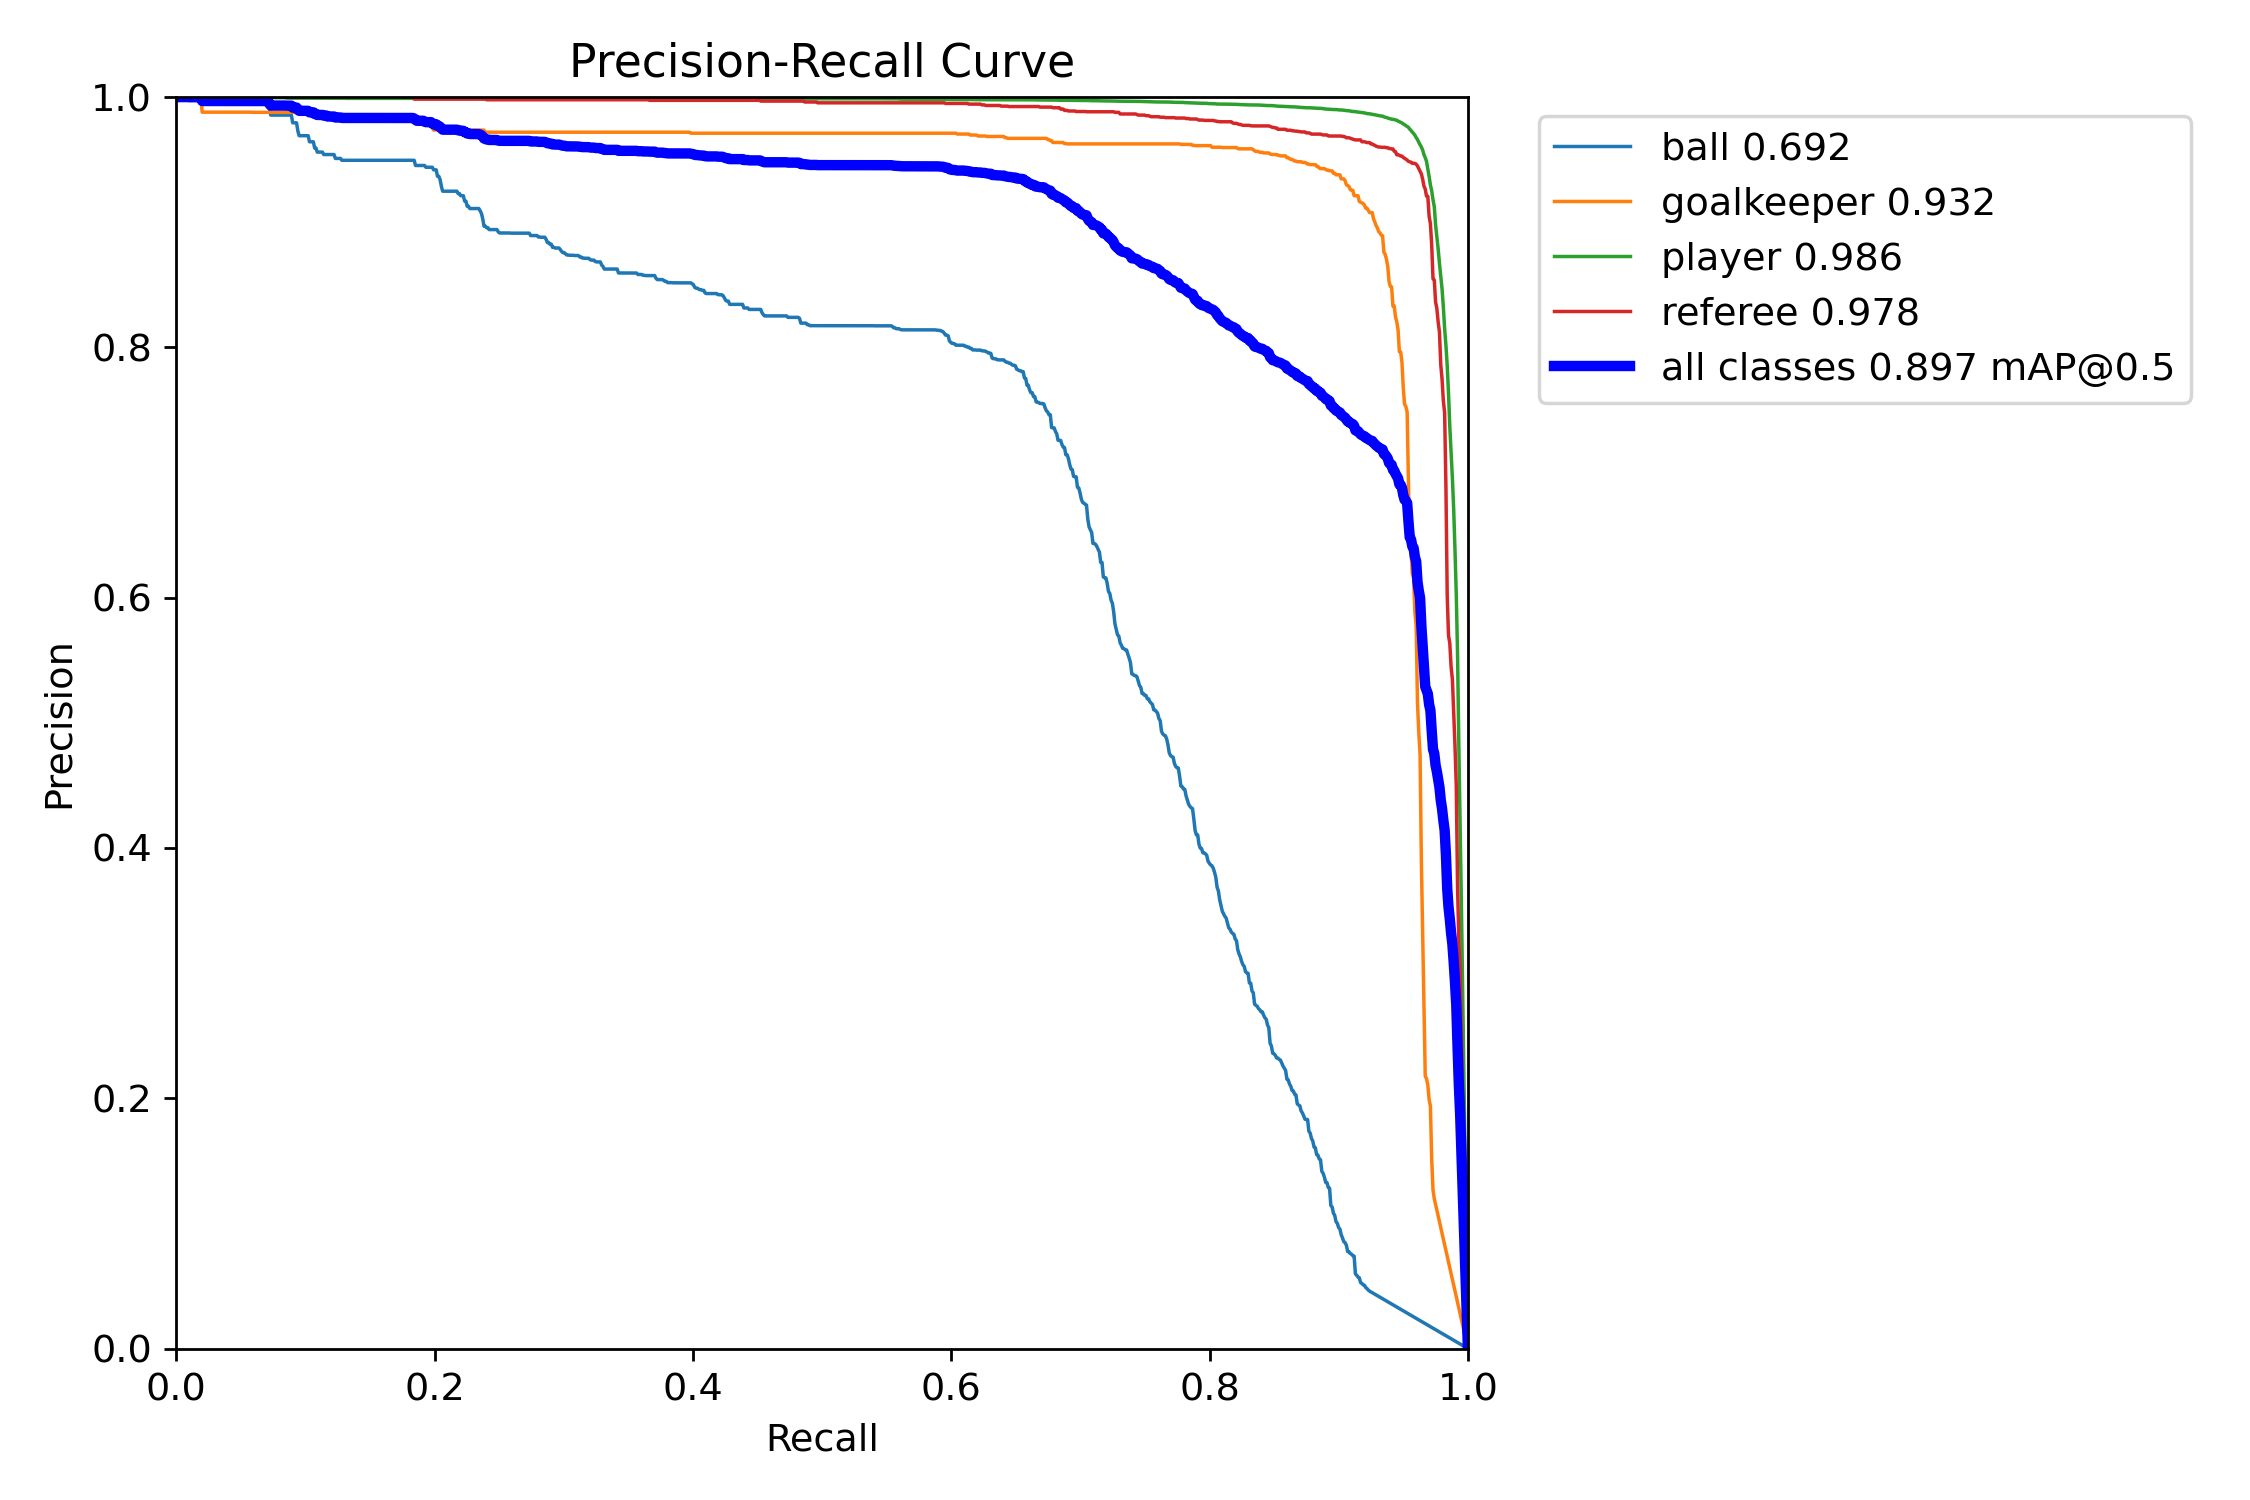
\includegraphics[width=.48\textwidth]{figures/Players Detection/PR_curve.png}\hfill
  
\includegraphics[width=.48\textwidth]{figures/Players Detection/confusion_matrix_normalized.png}
  \caption{Trái: đường cong Precision--Recall theo từng lớp. Phải: ma trận nhầm lẫn
           chuẩn hoá --- lớp \textit{ball} có tỉ lệ nhầm/bỏ sót cao nhất.}
\end{figure}

\begin{figure}[H]\centering
  
\includegraphics[width=.8\textwidth]{figures/Players Detection/val_batch0_pred.jpg}
  \caption{Ví dụ dự đoán của mô hình phát hiện trên một batch tập kiểm định.}
\end{figure}

\subsection{Mô hình keypoint sân (trên tập kiểm định)}
Mô hình keypoint đạt độ chính xác rất cao. Cần lưu ý tập kiểm định khá nhỏ (34 ảnh), nên
các con số này nên được xác nhận thêm trên dữ liệu đa dạng hơn trước khi kết luận tổng quát.

\begin{table}[H]\centering
\caption{Kết quả mô hình YOLOv11s-pose phát hiện keypoint sân.}
\begin{tabular}{lcc}
\toprule
Chỉ số & Box & Pose (keypoint) \\
\midrule
mAP@50            & 0.995 & 0.995 \\
mAP@50--95        & 0.984 & 0.813 \\
Precision / Recall & 1.0 / 1.0 & 1.0 / 1.0 \\
\bottomrule
\end{tabular}
\end{table}

\begin{figure}[H]\centering
  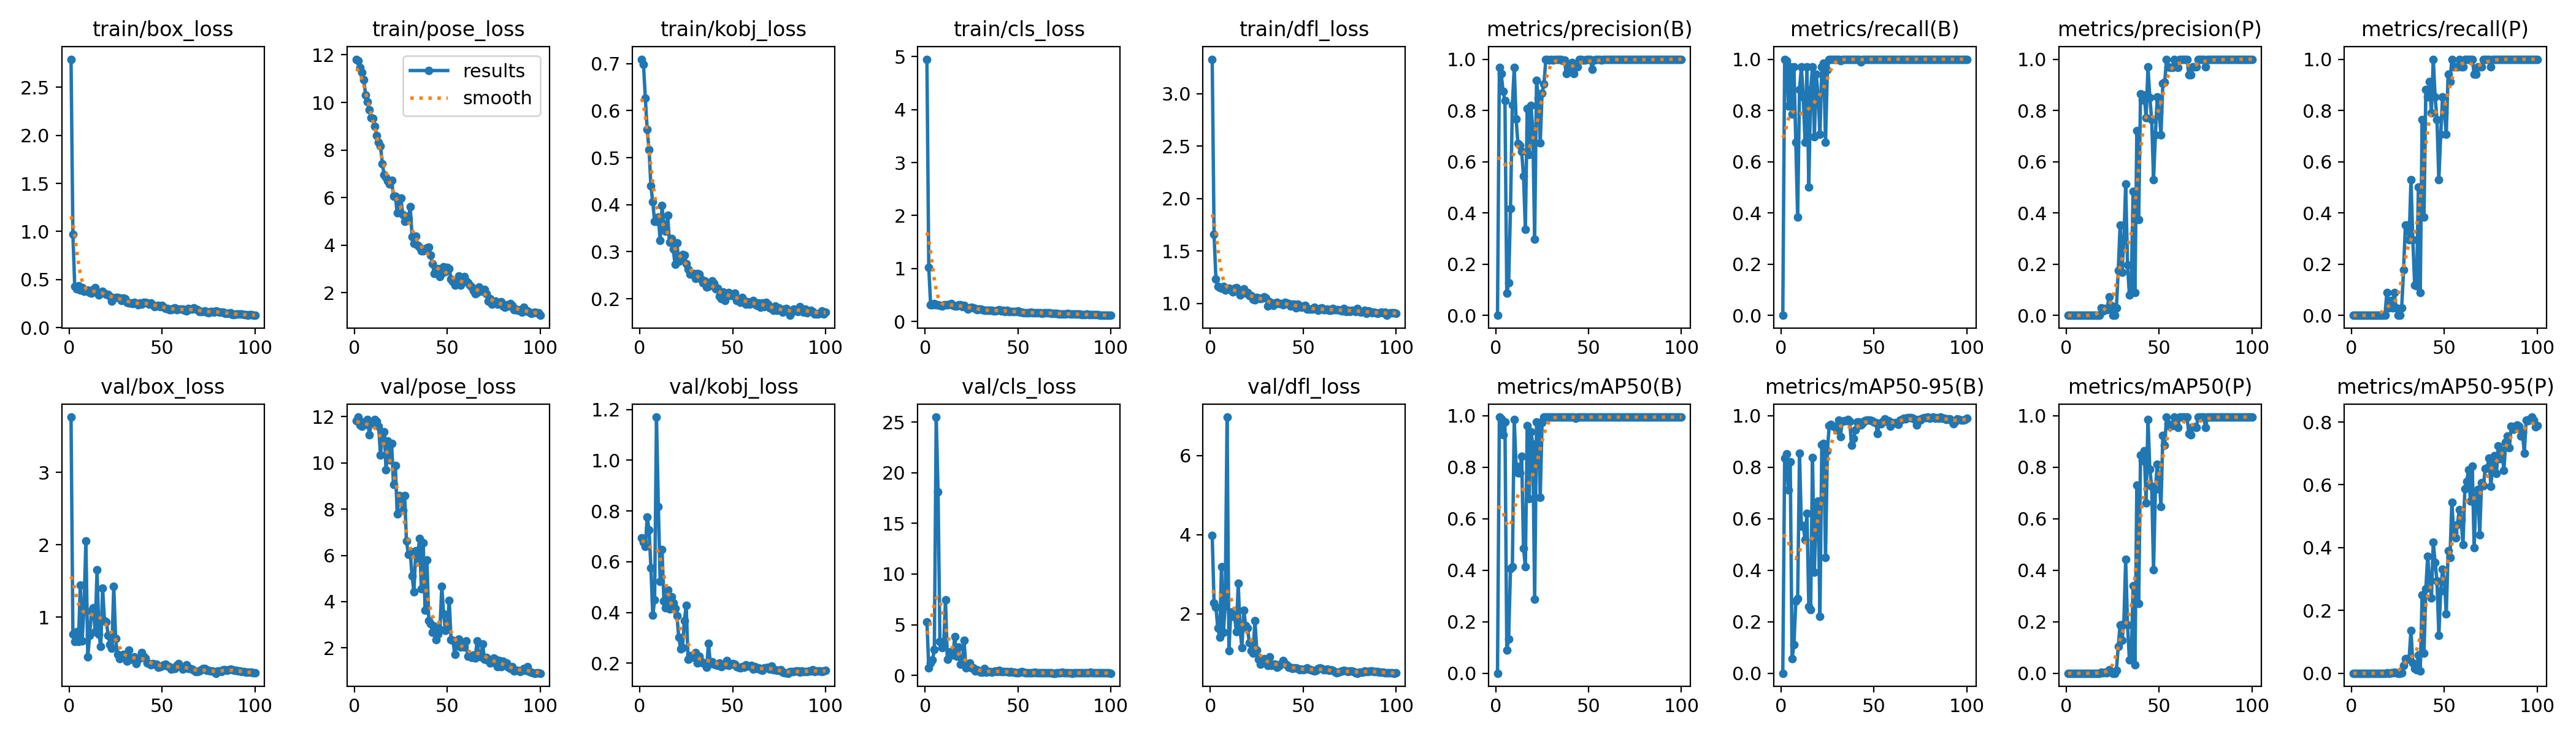
\includegraphics[width=\textwidth]{figures/Pitch Keypoint Detection/results.png}
  \caption{Quá trình huấn luyện mô hình keypoint sân (YOLOv11s-pose): loss box/pose
           giảm dần, các chỉ số mAP hội tụ ở mức rất cao.}
\end{figure}

\begin{figure}[H]\centering
  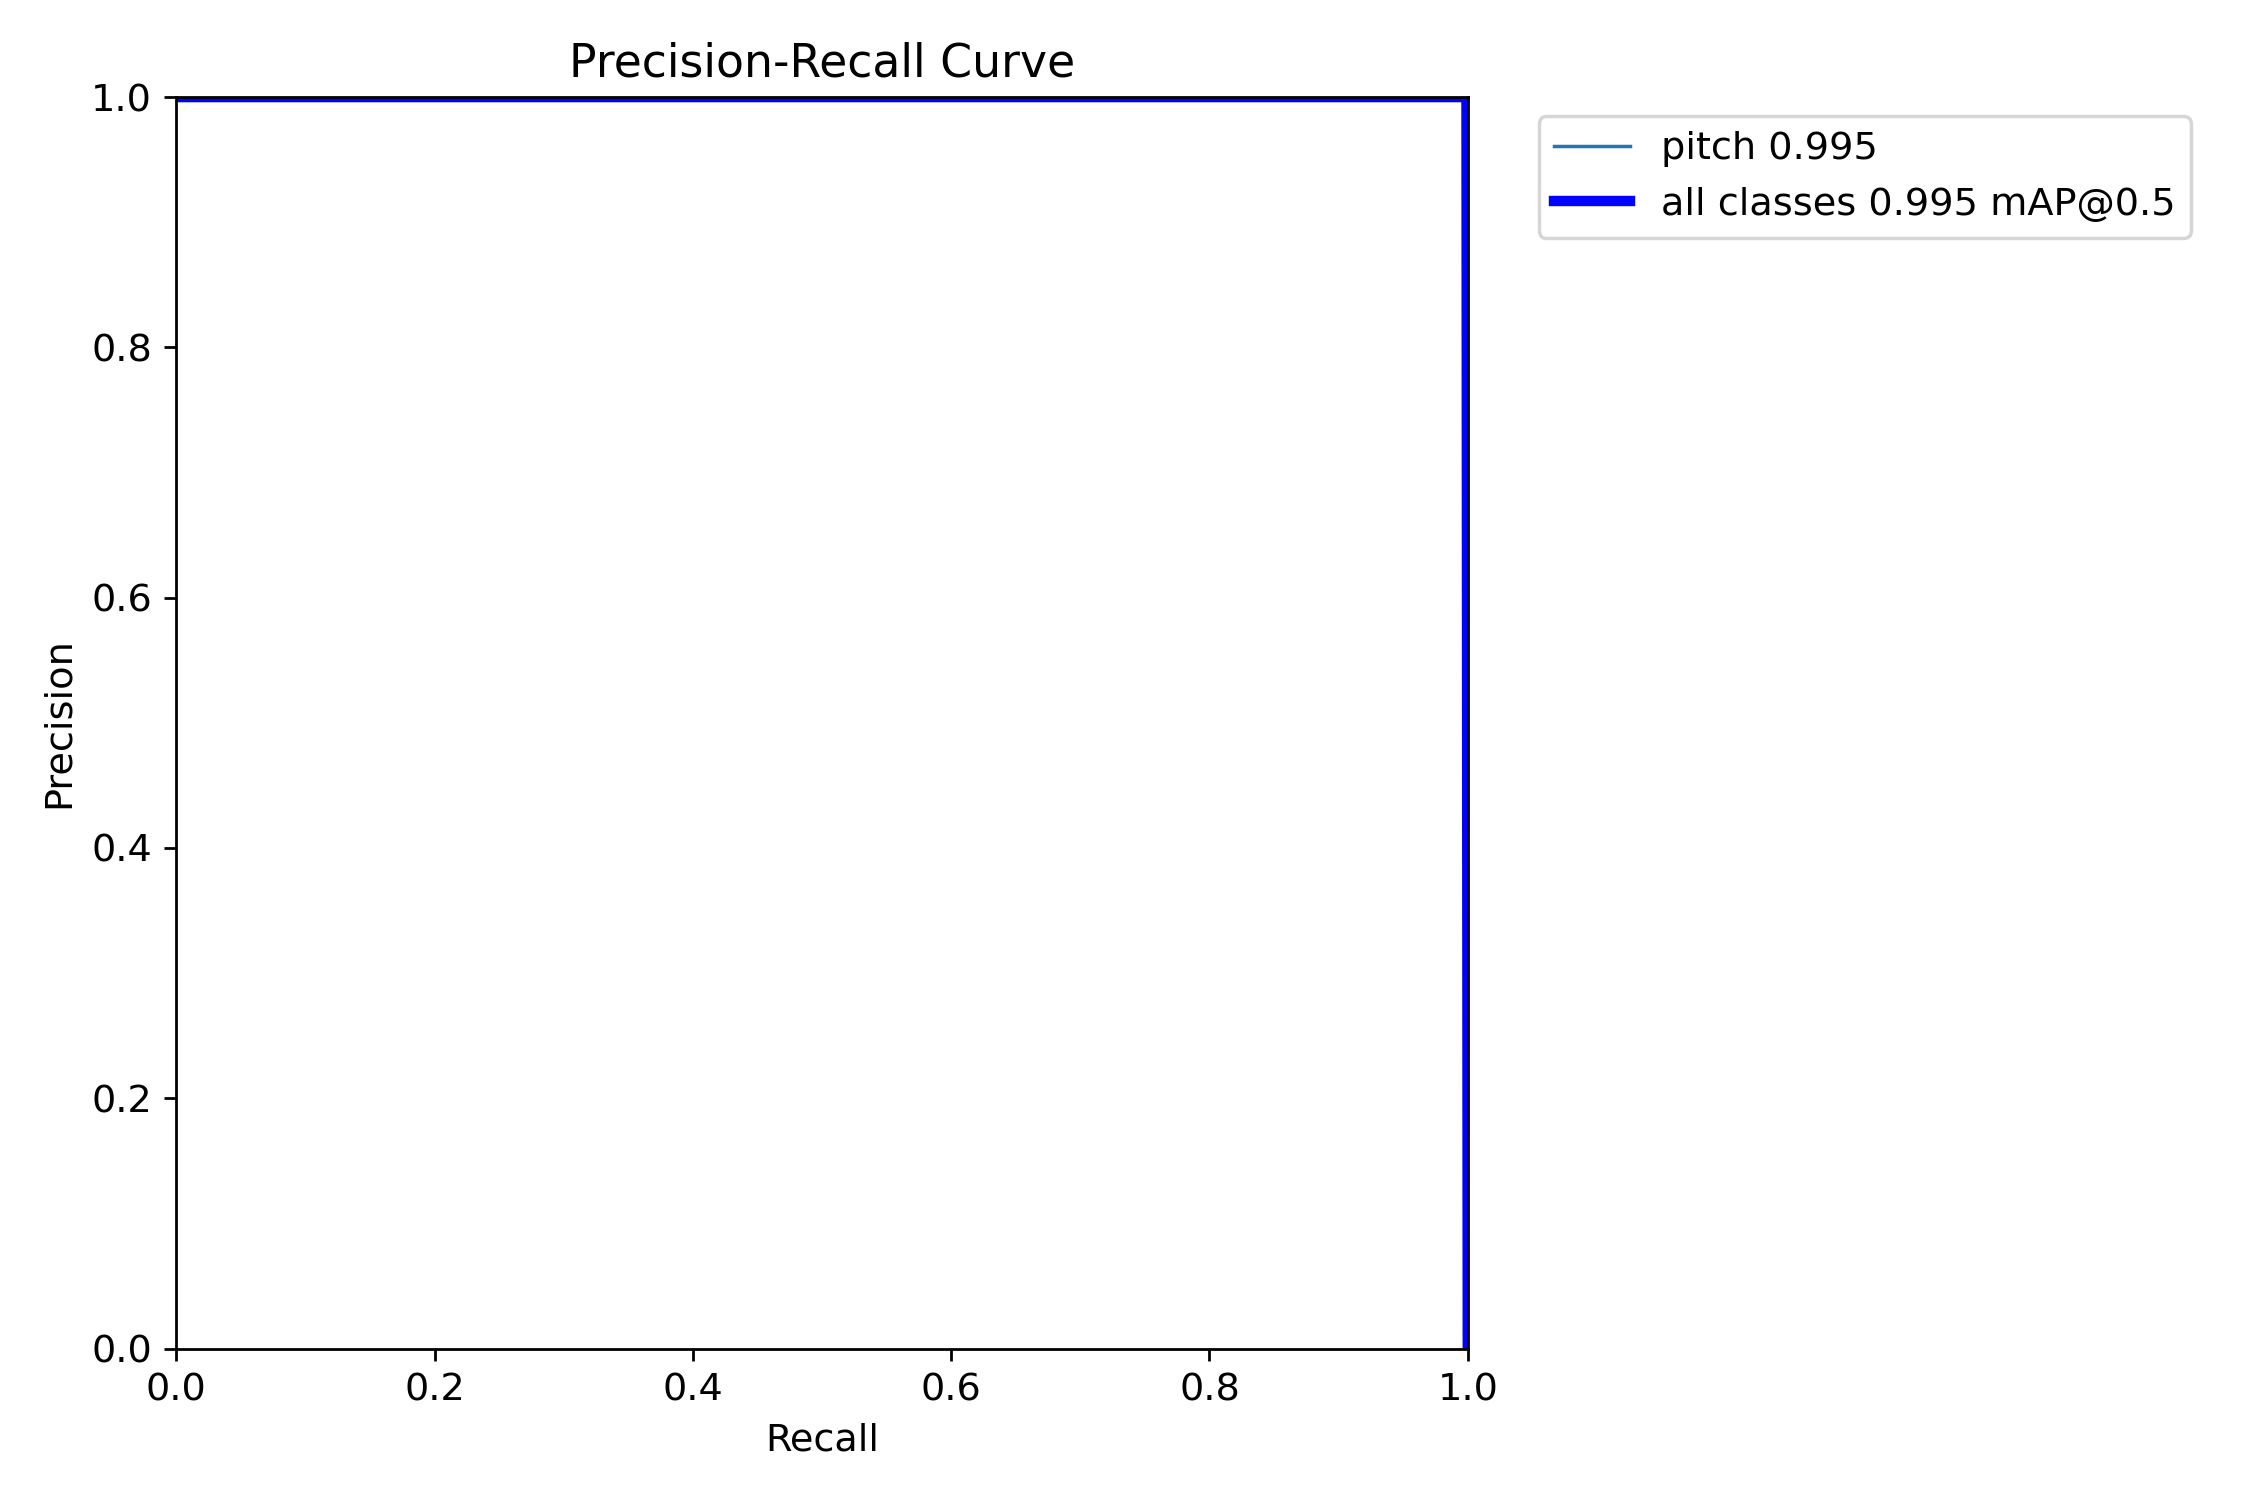
\includegraphics[width=.48\textwidth]{figures/Pitch Keypoint Detection/PosePR_curve.png}\hfill
  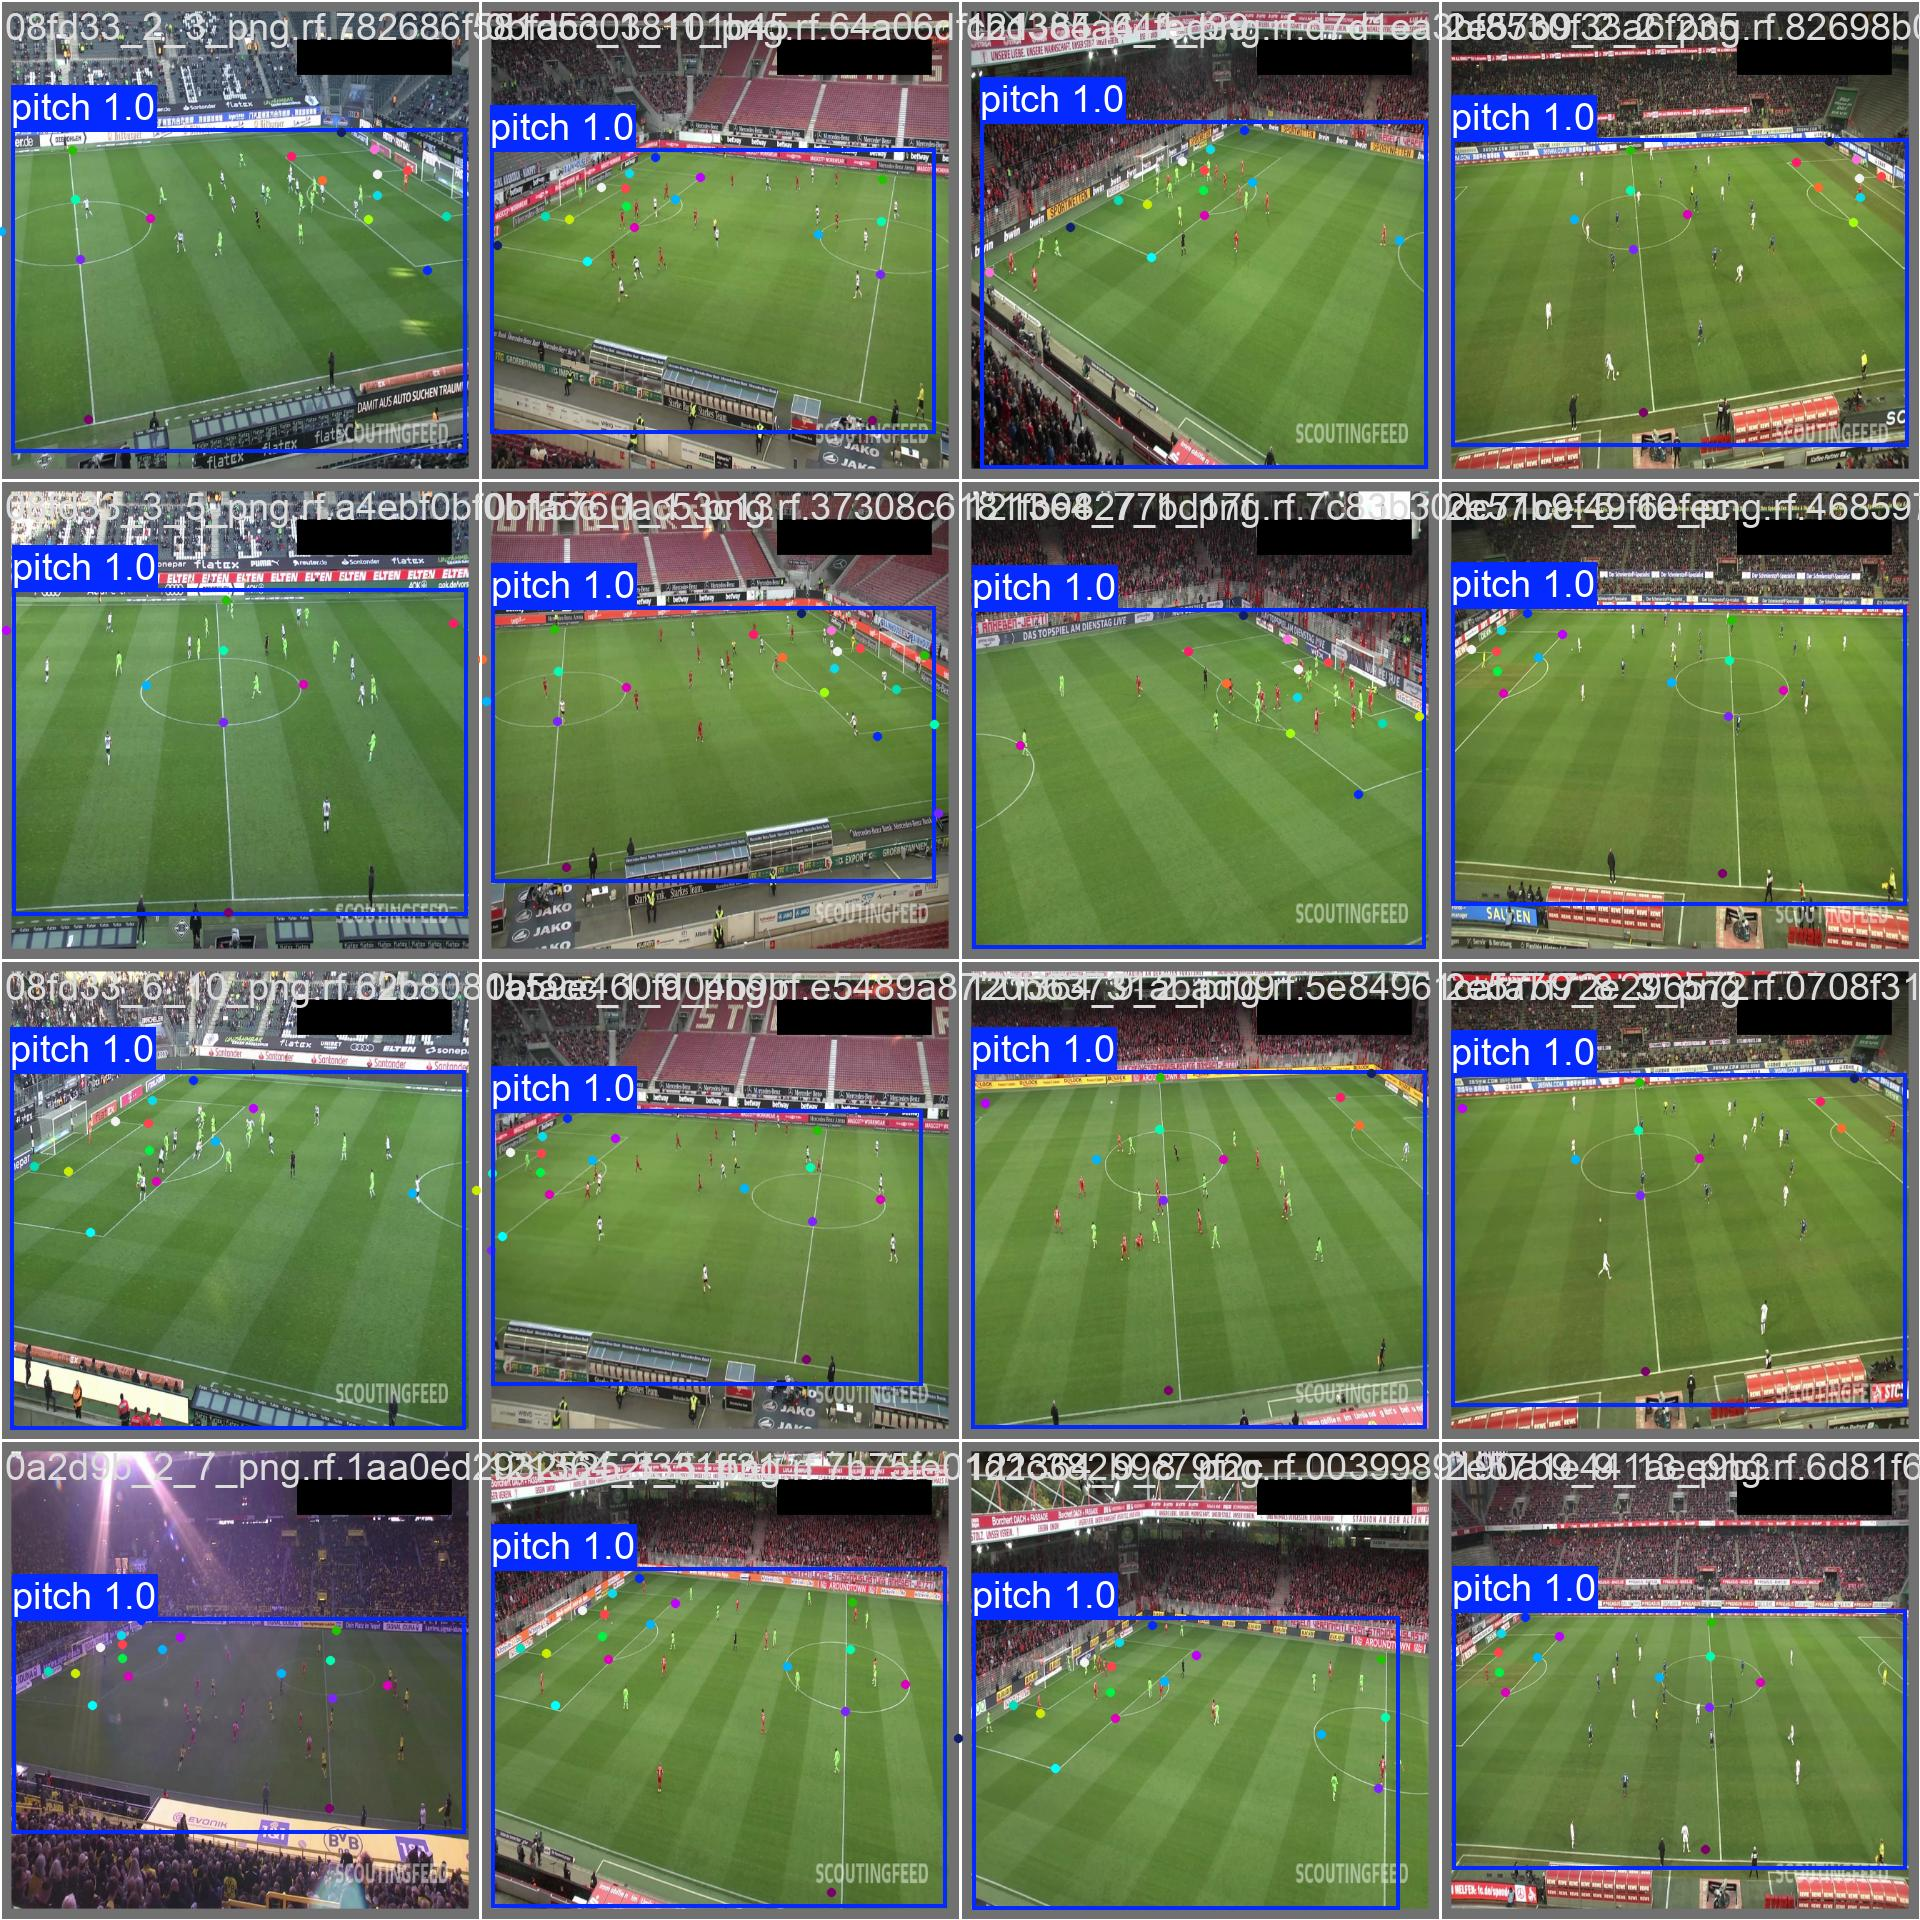
\includegraphics[width=.48\textwidth]{figures/Pitch Keypoint Detection/val_batch0_pred.jpg}
  \caption{Trái: đường cong Precision--Recall của bài toán keypoint (pose). Phải: ví dụ
           dự đoán 32 điểm mốc sân trên tập kiểm định.}
\end{figure}

\subsection{Phương pháp đánh giá định lượng toàn hệ thống}
\label{sec:eval}
Ngoài chỉ số của từng mô hình, hệ thống được đánh giá theo hai giao thức chuẩn, đối chiếu
với baseline GSR-Baseline của bộ dữ liệu SoccerNet Game State Reconstruction (SoccerNet-GSR):

\paragraph{Cách khuyến nghị --- GS-HOTA rút gọn.} GS-HOTA mở rộng từ HOTA, thay hàm tương
đồng IoU ảnh bằng tích $\mathrm{LocSim}\times\mathrm{IdSim}$, trong đó
\begin{equation}
  \mathrm{LocSim}(P,G)=\exp\!\Big(\ln(0{,}05)\,\tfrac{\lVert P-G\rVert_2^2}{\tau^2}\Big),\quad \tau=5\text{ m},
\end{equation}
là hạt nhân Gaussian trên khoảng cách (mét) giữa dự đoán $P$ và ground-truth $G$ trên sân,
còn $\mathrm{IdSim}=1$ khi mọi thuộc tính khớp. Vì pipeline \emph{không nhận diện số áo},
ta dùng biến thể $\mathrm{IdSim}$ chỉ xét \textbf{role + team} (bỏ jersey), tương ứng cấu
hình Pitch+Role+Team trong bảng ablation của paper. Bảng~\ref{tab:gshota} là khung so sánh.

\paragraph{Phương án dự phòng --- MOT ảnh.} Đánh giá thành phần theo dõi trong không gian
ảnh bằng HOTA/DetA/AssA/MOTA (Bảng~\ref{tab:mot}), đối chiếu Bảng S1 của paper.

Cả hai giao thức được hiện thực bằng một \emph{engine tự chứa} (module
\texttt{football\_analysis.evaluation}) đã được kiểm thử độc lập với dữ liệu (dự đoán hoàn
hảo cho HOTA\,$\approx$\,1, MOTA\,=\,1; $\mathrm{LocSim}(5\text{m})=0{,}05$), cùng hai
script \texttt{scripts/eval\_gsr.py} và \texttt{scripts/eval\_mot.py}. Các con số của
project (ô in đậm) được điền sau khi chạy trên tập SoccerNet tương ứng.

\begin{table}[H]\centering
\caption{So sánh GS-HOTA. Biến thể rút gọn (IdSim chỉ xét role+team, không jersey).}
\label{tab:gshota}
\begin{tabular}{lccccc}
\toprule
Phương pháp & Pitch & Role & Team & Jersey & GS-HOTA \\
\midrule
GSR-Baseline (test, đầy đủ)      & \checkmark & \checkmark & \checkmark & \checkmark & 22.26 \\
GSR-Baseline (valid, đầy đủ)     & \checkmark & \checkmark & \checkmark & \checkmark & 18.05 \\
Ablation Pitch+Role              & \checkmark & \checkmark & --         & --         & 40.76 \\
Ablation Pitch+Team              & \checkmark & --         & \checkmark & --         & 37.03 \\
\textbf{Hệ thống của đề tài}     & \checkmark & \checkmark & \checkmark & --         & \textbf{--} \\
\bottomrule
\end{tabular}
\end{table}

\begin{table}[H]\centering
\caption{So sánh MOT trong không gian ảnh (SoccerNet-Tracking, Bảng S1 của paper).}
\label{tab:mot}
\begin{tabular}{lcccc}
\toprule
Phương pháp & HOTA & DetA & AssA & MOTA \\
\midrule
ByteTrack (paper)      & 47.23 & 44.49 & 50.26 & 31.74 \\
GSR-Baseline (paper)   & 57.64 & 67.42 & 49.42 & 80.79 \\
FairMOT-ft (paper)     & 57.88 & 66.56 & 50.49 & 83.56 \\
\textbf{Hệ thống của đề tài (YOLOv11+ByteTrack)} & \textbf{--} & \textbf{--} & \textbf{--} & \textbf{--} \\
\bottomrule
\end{tabular}
\end{table}

\noindent\textit{Lưu ý trung thực:} bỏ jersey khiến bài toán định danh dễ hơn, nên số
GS-HOTA rút gọn không so ngang trực tiếp với 22.26 của baseline đầy đủ; cần đóng khung là
biến thể ``Pitch+Role+Team''.

\subsection{Kết quả hệ thống inference (định tính)}
Hệ thống đã chạy hoàn chỉnh trên cả ảnh lẫn video, tạo ra khung hình chú giải kèm radar 2D
và Voronoi hiển thị đồng thời, cùng tốc độ km/h dưới chân cầu thủ. Các vấn đề thực tế đã
được xử lý: sót cầu thủ ở xa do lệch độ phân giải suy luận; nhấp nháy nhãn đội; nhấp
nháy/mất dấu bóng (tự bắt lại và ẩn bóng khi mất dấu lâu); rung/lệch bản đồ do keypoint
(fit toàn bộ keypoint + cắt outlier, làm mượt có tâm rồi fit lại homography, bắc cầu quãng
mất sân bằng dead-reckoning); và quỹ đạo bóng bay bị vẽ cong trên bản đồ 2D.

\begin{figure}[H]\centering
  \includegraphics[width=.9\textwidth]{figures/ket_qua.png}
  \caption{Khung hình kết quả với radar 2D, biểu đồ Voronoi và tốc độ km/h.}
\end{figure}

% ============================ 6. HẠN CHẾ ============================
\section{Hạn chế và hướng phát triển}
\begin{itemize}[leftmargin=1.4em]
  \item Phát hiện bóng còn yếu nhất trong bốn lớp; có thể cải thiện bằng dữ liệu bổ sung,
        tăng độ phân giải, hoặc mô hình chuyên cho vật thể nhỏ.
  \item Ước lượng tốc độ và vị trí 2D phụ thuộc chất lượng homography từ một camera --- đây
        là \emph{ước lượng}, không phải đo lường chính xác; độ cao của bóng khi bay không
        khôi phục được từ một góc nhìn. Đo đạc cho thấy giới hạn hiện tại nằm ở độ chính xác
        định vị của mô hình keypoint: các keypoint tự mâu thuẫn nhau 10--22\,px một cách có
        hệ thống, tương đương lệch vài mét ở vùng xa cụm điểm neo --- không thuật toán hậu
        xử lý nào bù được vì sai lệch nằm ngay trong phép đo.
  \item Tập kiểm định keypoint nhỏ, nên đánh giá lại trên nhiều trận/sân khác nhau.
  \item \textbf{Hướng phát triển}: tiến tới ước lượng tham số camera bằng mạng học sâu huấn
        luyện trên dữ liệu lớn (hướng của các pipeline GSR đoạt giải SoccerNet) --- bền hơn
        khi chỉ thấy ít vạch sân lúc lia; khi có hiệu chỉnh camera đầy đủ thì khôi phục quỹ
        đạo bóng 3D bằng khớp parabol; bổ sung các chỉ số chiến thuật (cự ly đội hình,
        khoảng cách chuyền, kiểm soát khu vực) và tối ưu tốc độ để tiến gần thời gian thực;
        hoàn tất đánh giá định lượng ở mục~\ref{sec:eval} trên tập SoccerNet-GSR/Tracking.
\end{itemize}

\end{document}
